\section{Circuit Design}

The circuit design and schematic realization of the BRD1 sub-board of the device is discussed in the following sections. This includes sections on the DDS signal generator stage, the current driver stage, the output multiplexer, as well as discussions on power supplies, digital interfacing, and clock generation.

\begin{figure}
\centering
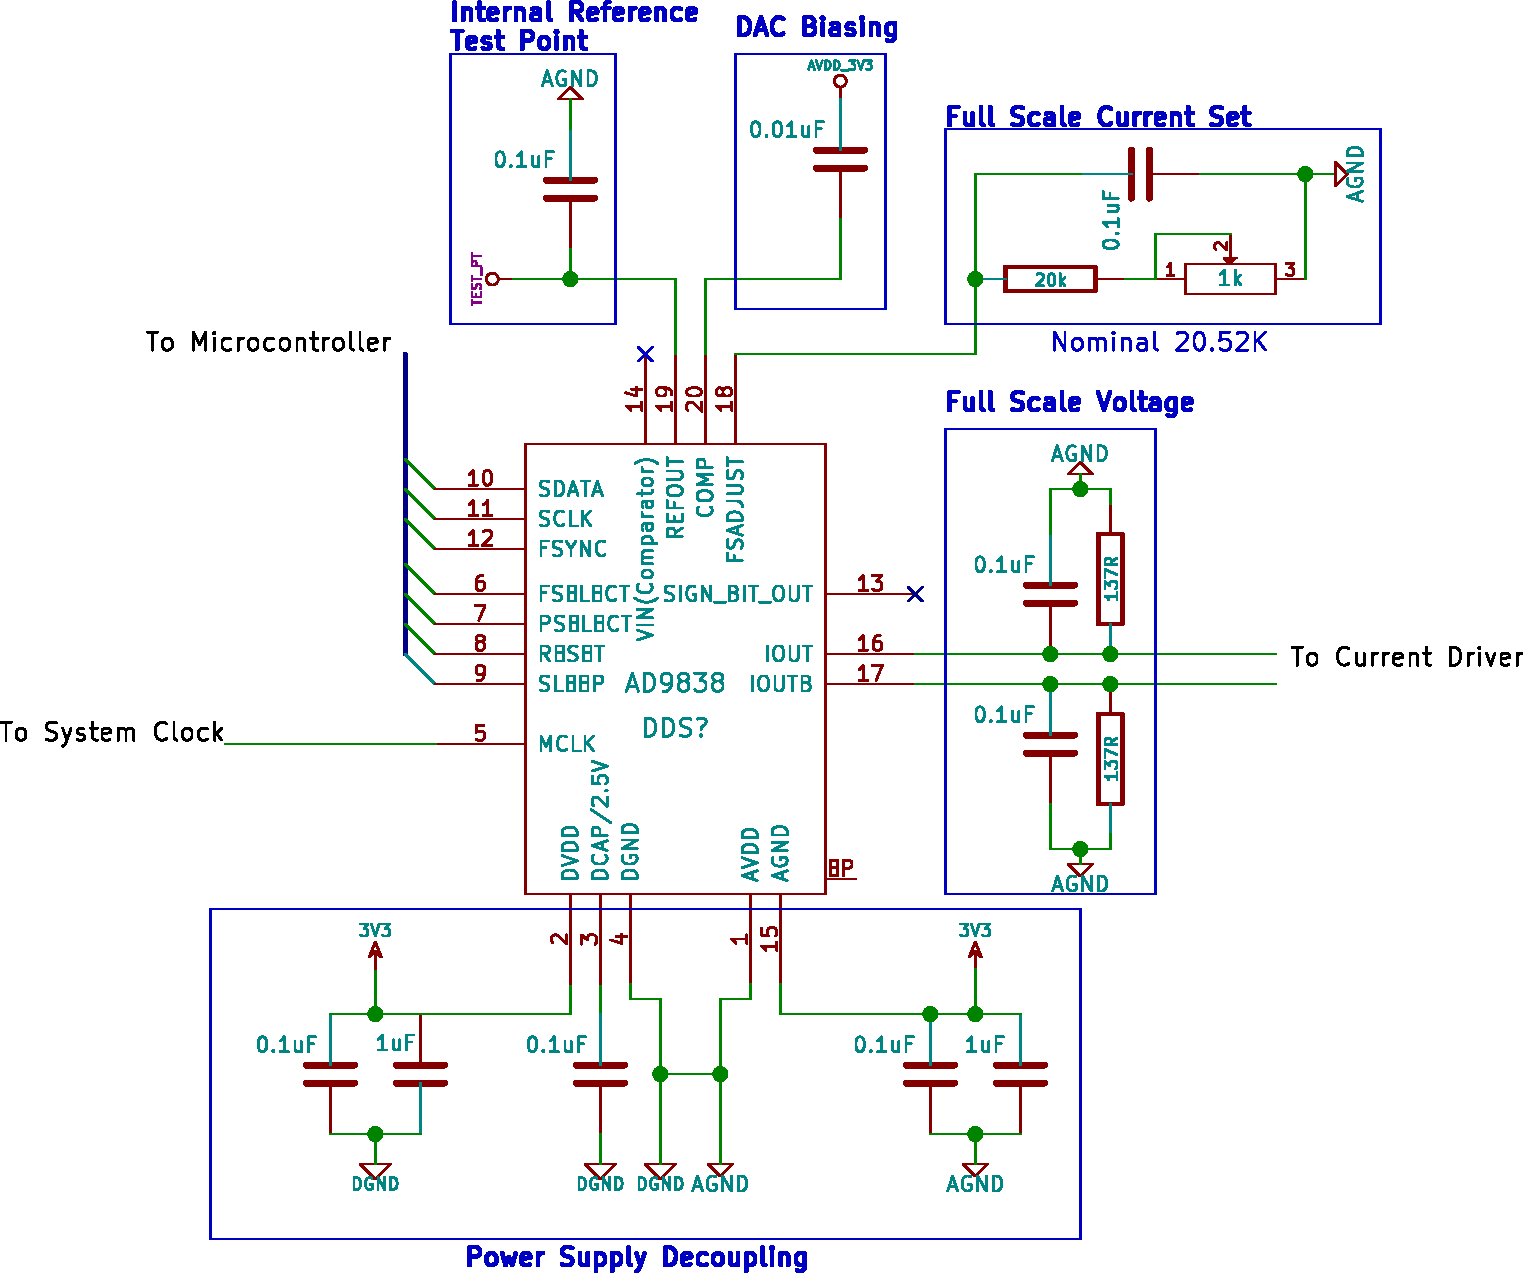
\includegraphics[width=0.9\textwidth]{../assets/images/DDS_Stage/DDS_stage_big}
\caption{Annotated schematic diagram of the DDS stage of the device. The AD9838 is the circuit element labeled DDS1. The pin names as well as pin numbers are indicated on the component.  Full Scale Current and Full Scale Voltage are used to set the input signal into the current driver stage, the functionality is discussed in Section \ref{sec:circuit_subs:dds_stage}. Power Supply decoupling is required for all power supply pins in order to minimize spurious pcb and power supply noise from bleeding into the signal, decoupling best practices are discussed in Section \ref{sec:pcb_subs:decoupling}. The internal reference pin outputs the an internal voltage referense used by the DDS, used in this design as a test point. }
\label{fig:dds_stage_main_fig}
\end{figure}


\subsection{DDS Stage}
\label{sec:circuit_subs:dds_stage}


\newthought{The first element in the TDCS driver signal stage} is the {\bf D}irect {\bf D}igital {\bf S}ynthesis ({\bf DDS}) device. The DDS replaces a microcontroller and a {\bf D}igital-{\bf A}nalog Convert ({\bf DAC}) to produce sinusoidal and triangular voltage signals in a single device.  The DDS device is designed by the manufacturer to produce a fixed signal at a digitally selectable frequency, this limits possible output options, but the integrated design limits noise, power, and reduces component count vs a discrete system. A DDS works by increasing the number stored in a register (phase accumulator) with every clock cycle, the number stored in the accumulator is used to lookup a code stored in a static "lookup table" that corresponds to the output code for the integrated DAC. By changing the size of the numerical jump that the phase accumulator undergoes every clock cycle, you can adjust the frequency through a digital "control word". 

\begin{marginfigure}
\framebox{\begin{minipage}[t]{1\columnwidth}
\end{minipage}}
insert figure here

\end{marginfigure}



There are a variety of DDS components on the market, they are differentiated by primarily by type and number of outputs, its noise profile, the frequency limits, power consumption, and bit depth \sidenote[][]{There are two bit depths that are important from a design perspective. The phase accumulator bit depth (the number of discrete steps to complete one cycle) determines the frequency resolution of the DDS. The DAC output bit depth determines the number of discrete "output modes" that the DDS can utilize to produce a signal. Typically the DAC bit depth is smaller than the phase accumulator, this means that the DDS may output the same voltage for several sequential phase steps which creates phase noise} There are also a number of other features that could be useful in certain applications, but were not considered for this implementation. For further discussion of DDS component selection refer to Section \ref{sec:components_subs:AD9838} 

Providing an output current that can both be negative or positive relative to local ground can be accomplished in several different ways. DDS outputs can either be bipolar, complimentary, or single ended, each requiring a different type of output coupling to achieve true bipolar output (see Section\ref{sec:components_subs:AD9838} for more information). The AD9838 provides complimentary current outputs, which allows for higher speeds than a voltage-output dds, and conveniently couples to the current driver stage (see Section \ref{sec:circuit_subs:vtoi}) to provide a symmetrical output signal. Complimentary current DDS devices supply the output waveform on two seperate pins (OUTA and OUTB), as the phase accumulator progresses through the steps, the output on OUTA increases from I$=0$ to $\text{I} = \text{I}_\text{Full Scale}$ while the output on OUTB decreases from $\text{I} = \text{I}_\text{Full Scale}$ to $\text{I} = 0$ over the same interval\sidenote[][]{The full scale current of the AD9838 is set with an external resistor, following the equation $\text{I}_\text{Full Scale} = 18 \times \frac{1.14\text{V}}{\text{R}_\text{ set}(\text{k}\Omega)}.$ With $\text{R}_\text{ set} = 20.52 \text{k}\Omega$, $\text{I}_\text{Full Scale} = 1\text{mA}$}. By taking the difference between these two outputs, a full bipolar output can be reconstructed from a single-ended (only positive voltages) complimentary DDS. A partial schematic of the AD9838 and supporting components is shown in Fig \ref{fig:dds_stage_main_fig}

This complimentary current output must be voltage coupled in order to work with the high input-impedance driver stage. This is accomplished by placing a resistor from the current output to ground, using Ohm's law and the given full-scale current, the full-scale voltage can be easily calculated for a given shunt resistor (In this design, $1\text{mA}$ across $137\Omega$ gives $.137\text{V}$ Peak). The AD9838 can operate within specification (output compliance) at output levels of up to $0.8\text{V}$ Peak.

Digital Control lines are used to interface with the device. The AD9838 has 3 lines dedicated to serial communication (Indicated in Fig. \ref{fig:dds_stage_main_fig} as {\bf~SDATA}, {\bf~SCLK}, and {\bf~FSYNC}) which are used for loading frequency control words and otherwise setting the operating parameters of the device. The {\bf~FSELECT} and {\bf~PSELECT} pins allow for rapid switching between stored frequencies and phase offsets (this functionality can be achieved through the serial data lines but at a much lower switching rate). {\bf~SLEEP} and {\bf~RESET} control the power state of the device. {\bf~MCLK} is the digital sampling clock input for the AD9838 (clock source is discussed in Section \ref{sec:circuit_subs:clock} )

All integrated circuits used are required to be decoupled from the power supply through the use of decoupling capacitors (capacitors placed between the power supply pin and ground) that filter high frequency noise and other unwanted spurious noise that can leak through the power supply. Power Supply decoupling is discussed in Section \ref{sec:pcb_subs:decoupling}



